\documentclass[paper=a4, fontsize=12pt]{scrartcl}
\usepackage[T1]{fontenc} 
\usepackage[english]{babel}
\usepackage{amsmath,amsfonts,amsthm}
\usepackage{pxfonts}
\usepackage{units}
\usepackage{url}
\usepackage[pdftex]{graphicx}
\usepackage{listings}
\graphicspath{{./img/}}
\DeclareGraphicsExtensions{.pdf,.jpeg,.png}
\usepackage{cite}

\title{	
  \rule{\linewidth}{1px} \\[0.4cm]
  \textsc{Computer-Aided Verification} \\ [25pt]
  \huge Project report \\
  \rule{\linewidth}{1px} \\[0.4cm]
  \textsc{Boehm Simon} \\ [12pt]
  \textsc{Danger Daniel} \\ [12pt]
  \textsc{Roob Julius} \\ [12pt]
  \rule{\linewidth}{1px} \\[0.4cm]
}

\begin{document}
\maketitle 

\section{Introduction}
In a short sentences the goal of our project is the re-implementation of the Boogie verification condition generator. 



Boogie is a Intermediate Verification Language published by Microsoft Research which is designed to make the prescription of verification conditions natural and convenient. The architecture of Boogie is build to verify Spec\# programs in the object oriented .Net framework. This is done by a pipeline performing a series of transformations from the source program in Spec\# over Boogie and verification conditions to an error report. This pipline is shown in figure \ref{fig:pipline}

\begin{lstlisting}[caption=Boogie program example, label=lst:example]
procedure Find(a: int, b: int) returns (k: int)
  requires a <= b;
  requires (forall j: int :: a < j && j < b ==> f(j) != K);
  ensures f(k) == K;
{
  // nondeterministically choose one of these 3 goto targets
  goto A, B, C;  

  A:
    // assume we get here only if 'f' maps 'a' to 'K'
    assume f(a) == K;  
    k := a;
    return;

  B:
    // assume we get here only if 'f' maps 'b' to 'K'
    assume f(b) == K;  
    k := b;
    return;

  C:
    // neither of the two above
    assume f(a) != K && f(b) != K;  
    call k := Find(a-1, b+1);
    return;
}
\end{lstlisting}

Our goal is the part of this pipeline where the verification conditions are generated from the Intermediate Verification Language Boogie. This can be divided into two sub-parts: the parsing of the Boogie program code and the generation of verification conditions. The verification conditions should then be solved by a SMT solver, e.g. Z3.

We decided to use Python as programming language for this project, because it overs a lot of great and easy to use libraries. 

\begin{figure}[ht]
  \centering
    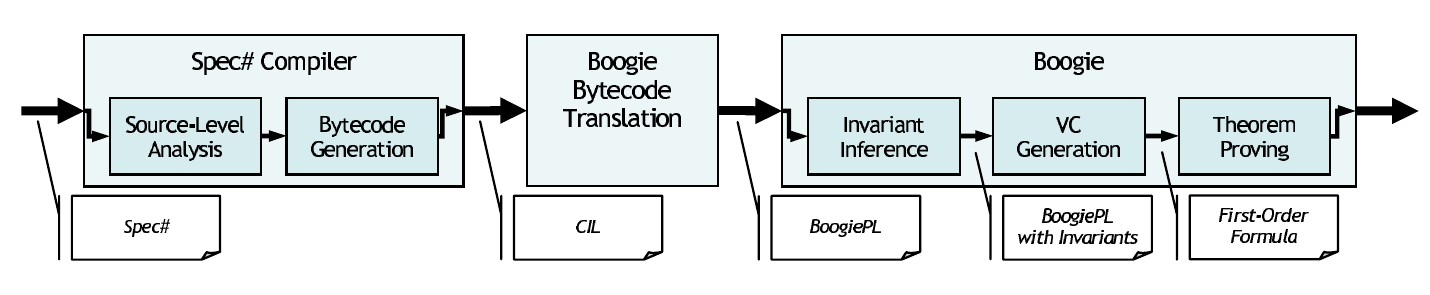
\includegraphics[height=3cm]{pipline}
    \caption{The Boogie pipline \cite{boogie}.}
  \label{fig:pipline}
\end{figure}

There are mainly two Boogie papers. "This is Boogie 2"\cite{boogie2} and "Boogie: A Modular Reusable Verifier for Object-Oriented Programs"\cite{boogie}. For our work "This is Boogie 2" is the main source because it contains the whole grammar and semantics of the Boogie language."Boogie: A Modular Reusable Verifier for Object-Oriented Programs" describes more the techniques used to convert Spec\# sources to Boogie programs, which is not part of our project. Another source is the source code of the Boogie implementation from Microsoft Research, which is available under the Microsoft Public License (Ms-PL). But because there are a lot of additional features the code is hard to understand and not easy to reuse for our purposes.

\section{Parsing}
For the parsing of Boogie programs the Python package PLY is used. PLY stands for Python Lex-Yacc and is the Python implementation of the compiler construction tools ley and yacc. Lex is used to generate a lexical analyser, a so called lexer, which divides the Boogie source code into single tokens and yacc is used to generate the parser. 

\begin{figure}[ht]
  \centering
    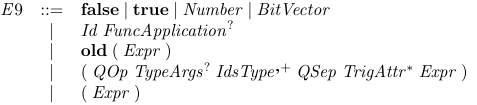
\includegraphics[height=3cm]{e9}
    \caption{A single Boogie grammar rule \cite{boogie2}.}
  \label{fig:e9}
\end{figure}

The implementation of the parser costs most the time because the conversion of all the Boogie grammar rules was very time-consuming and error-prone. Figure \ref{fig:e9} shows such a rule and listing \ref{lst:e9} shows a part of the corresponding code

\begin{lstlisting}[caption=Boogie program example, label=lst:e9]
def p_E9_number(p):
''' E9 : NUMBER '''
p[0] = Number(p[1])

def p_E9_id(p):
'''E9 : ID
      | ID '(' ')'
      | ID '(' exprlist ')' '''
if len(p) == 2:
p[0] = Variable(p[1])
else:
pass 

def p_E9_bool(p):
'''E9 : FALSE
      | TRUE '''
if p[1] == 'true':
p[0] = Boolean('true')
else:
p[0] = Boolean('false')	


def p_E9(p):
'''E9 : BITVECTOR
      | OLD '(' expr ')'
      | '(' FORALL typeargs idstypelist QSEP expr ')'
      | '(' FORALL idstypelist QSEP expr ')'
      | '(' EXISTS typeargs idstypelist QSEP expr ')'
      | '(' EXISTS idstypelist QSEP expr ')'
      | '(' FORALL typeargs idstypelist QSEP trigattr expr ')'
      | '(' FORALL idstypelist QSEP trigattr expr ')'
      | '(' EXISTS typeargs idstypelist QSEP trigattr expr ')'
      | '(' EXISTS idstypelist QSEP trigattr expr ')' '''
pass

def p_E9_bracket(p):
'''E9 : '(' expr ')' '''
p[0] = p[2]
\end{lstlisting}

\section{Verification}
After the parser was been implemented an abstract syntax tree (AST) from the program was build. But because Boogie is a very comprehensive language we decide to implement at first only the important part of the language in the AST to get a simple program to work. Figure \ref{fig:ast} shows such an AST.

\begin{figure}[ht]
  \centering
    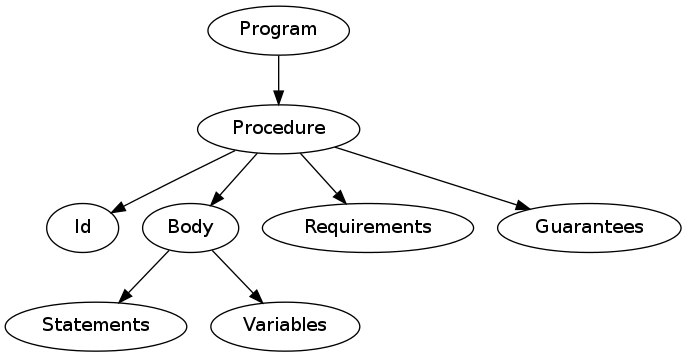
\includegraphics[height=4cm]{ast}
    \caption{Abstract syntax tree.}
  \label{fig:ast}
\end{figure}

For the verification formulas for each variable assignments are generated. Listing \ref{lst:ver} shows an example how this will look like for a simple Boogie program.
  
\begin{lstlisting}[caption=Formula generation, label=lst:ver, mathescape]
procedure p(z:int) 
{ 
  requires z>=3;      $E = {z_0 >= 3}$ 
  var x:int; 
  x = 2;              $E = E \cup {x_0 = 2}$ 
  x = x+z;            $E = E \cup {x_1 = x_0 + z_0}$ 
  assert x < 42;      $SAT(E \wedge \neg(x_1 < 42)) $ 
} 
\end{lstlisting}

At the point $SAT(E \wedge \neg(x_1 < 42))$ the formula is given to the SMT solver Z3. We decided to use Z3 because it is easy to use out of Python.

% TODO insert output of z3

\section{Conclusion}
% TODO bla blub interesantes project blub wenig zeit bla..... 


\bibliographystyle{alpha} 
\bibliography{literature}

\end{document}

